
\chapter{The ATLAS Experiment at the Large Hadron Collider}
\label{chap:experiment}
%To test the theoretical predictions of the Standard Model, huge experimental setups with unprecedented size and complexity are required.
The ATLAS experiment~\cite{PERF-2007-01} is a multipurpose detector that measures the particle-particle collisions produced by the \emph{Large Hadron Collider} (LHC)~\cite{Evans:2008zzb} with extreme precision. It is designed to measure a broad range of physics processes, with a focus on providing more insight into the Higgs boson.
The LHC is the world's most powerful particle accelerator to date. It remains the most recent large-scale upgrade to the accelerator complex at CERN, the \emph{European Organization for Nuclear Research}, and produces collision events at unprecedented energies.
This chapter first provides an overview of the LHC, followed by a detailed description of the various aspects of the ATLAS experiment.

\section{The Large Hadron Collider}
%The two major technical components are \emph{radiofrequency cavities} (RF cavities) with oscillating electromagnetic fields to accelerate the particles as well as organizing them in so-called \emph{bunches}\footnote{RF cavities oscillate at a given frequency. Particles arriving early (late), will be decelerated (accelerated) so that the particles are kept together in discrete packages called bunches.} and magnet systems to bend, steer, and focus the particles' trajectories. The peak particle energy reached by a hadron collider is thereby limited by the maximum field strength of the bending magnets.
The LHC was designed and built for more than two decades starting in the early 1980s by more than $10000$ international researchers, engineers, and technicians from more than $100$ different countries.
The LHC is located in a near-circular tunnel\footnote{The same tunnel was used by the former LEP collider~\cite{LEPDesignReport}.} an average of \SI{100}{\m} below the France-Switzerland border close to Geneva (Switzerland). It has a circumference of \SI{26.7}{\km} and in its main mode of operation collides protons\footnote{The LHC also produces heavy-ion collisions in dedicated running periods} with a centre-of-mass energy of $\comEn = \SI{13}{\TeV}$\footnote{The LHC design centre-of-mass energy is $\comEn = \SI{14}{\TeV}$.}.
The protons are accelerated with 16 \emph{radiofrequency cavities}, that have oscillating electromagnetic fields and group the protons in \emph{bunches}\footnote{The radiofrequency cavities oscillate at a design frequency of \SI{400}{\mega\hertz}. The particles that arrive early (late), are decelerated (accelerated) so that the particles are kept together in discrete packages called bunches.}.
These bunches occupy two separate but nearby rings to form counter-rotating particle beams.
The LHC is designed to contain a maximum of 2808 bunches that are separated by a bunch spacing of \SI{25}{\ns}. Each bunch consists of about \SI{e11}{protons} which results in a design instantaneous luminosity of $\instLumi = \SI{e34}{\per\cm\per\s}$.\footnote{The machine and beam parameters of the LHC can vary between different data-taking cycles. More details can be found in \cref{sec:run-2-data-taking}.}
More than 1200 superconducting dipole magnets are used to force the particle beams on a curved trajectory.
They are designed to reach field strengths of up to \SI{8.33}{\tesla}, enabling the unprecedented collision energies\footnote{The peak particle energy reached by a hadron collider is limited by the maximum field strength of the bending magnets.}. More than 400 quadrupole magnets are used to focus the beams and increase the particle density within each bunch, which is especially important before the beams collide at any of the four main \emph{interaction points} (IPs). Each IP is surrounded by large detector systems that are optimized and designed for different physics objectives.
The ATLAS\footnote{A Toroidal Lhc ApparatuS} and CMS\footnote{Compact Muon Solenoid}~\cite{CMS-TDR-08-001} experiments are multipurpose detectors, designed to measure a large variety of physics processes. The LHCb\footnote{Large Hadron Collider beauty} experiment~\cite{1748-0221-3-08-S08005} is dedicated to measuring processes that involve $b$-quarks and ALICE\footnote{A Large Ion Collider Experiment}~\cite{1748-0221-3-08-S08002} focuses on the analysis of heavy-ion collisions.\footnote{There are other smaller experiments operating at the LHC: the TOTEMd (Total Elastic and Diffractive Cross Section Measurement)~\cite{1748-0221-3-08-S08007} and LHCf (Large Hadron Collider forward)~\cite{1748-0221-3-08-S08006} experiments study scattering processes close to the beam line and the MoEDAL (Monopole and Exotics Detector at the LHC) experiment~\cite{1742-6596-631-1-012014} is dedicated to the search for magnetic monopoles.}

Before the protons enter the LHC, they pass through a series of smaller accelerators. A schematic of the entire accelerator complex is shown in \cref{fig:accelerator-complex}.
The protons are extracted by ionising hydrogen atoms and first accelerated in the linear accelerator \emph{Linac2} (Linear accelerator 2)\footnote{Starting in 2020, Linac2 will be replaced by a new linear accelerator, Linac4 (Linear accelerator 4). More information can be found in \ccite{CERN-AB-2006-084}.}. Three synchrotrons follow: the \emph{BOOSTER} (Proton Synchrotron Booster), the \emph{PS} (Proton Synchrotron), and the \emph{SPS} (Super Proton Synchrotron).
They have an increasingly larger circumference and gradually increase the energy of the proton beams.
The proton beams from the SPS are finally injected into the LHC with an energy of $450\,\GeV$. The filling and ramp-up phases until stable beams are brought to collision at their final energies take around 45 minutes. The experiments at the LHC record the collision events for ideally about 8-10 hours or more, until the intensity of the beams becomes too low, making it more efficient to dump the beam and start a new cycle.

The operation of the LHC is broken down into different runs that last several years with differing running conditions.
\Cref{tab:lhc-lumi-overview-years} shows basic characteristics of the $pp$ collisions produced in so-called \RunOne and \RunTwo of the LHC, that occured between 2011-2012 and 2015-2018, respectively. After a technical shutdown between 2018 and 2022, the LHC is expected to continue to operate with \RunThr at a centre-of-mass energy \TDnote{of}{check again later} $\sqrt{s} = \SI{13.6}{\TeV}$.
Details on the \RunTwo data taking period and the performance of the ATLAS data acquisition are given in \cref{sec:run-2-data-taking}.

\FloatBarrier

\begin{table}[t]
  \centering
  \begin{tabular}{l | c | rr}
    \toprule
                             & Year      & \comEn [\TeV] & \intLumi [\ifb] \\
    \midrule
    \multirow{2}{*}{\RunOne} & 2011      & 7             & 5.5             \\
                             & 2012      & 8             & 22.8            \\
    \midrule
    \multirow{4}{*}{\RunTwo} & 2015      & 13            & 4.2             \\
                             & 2016      & 13            & 38.5            \\
                             & 2017      & 13            & 50.2            \\
                             & 2018      & 13            & 63.3            \\
    \midrule
    Full \RunTwo             & 2015-2018 & 13            & 156.2           \\
    \bottomrule
  \end{tabular}
  \caption{
    Summary of the centre-of-mass energy and integrated luminosity delivered by the LHC in $pp$ collisions during \RunOne and \RunTwo.}
  \label{tab:lhc-lumi-overview-years}
\end{table}

% Taken from \ccite{PublicLumiResults,PublicLumiResultsRun1}.




\begin{figure}
    %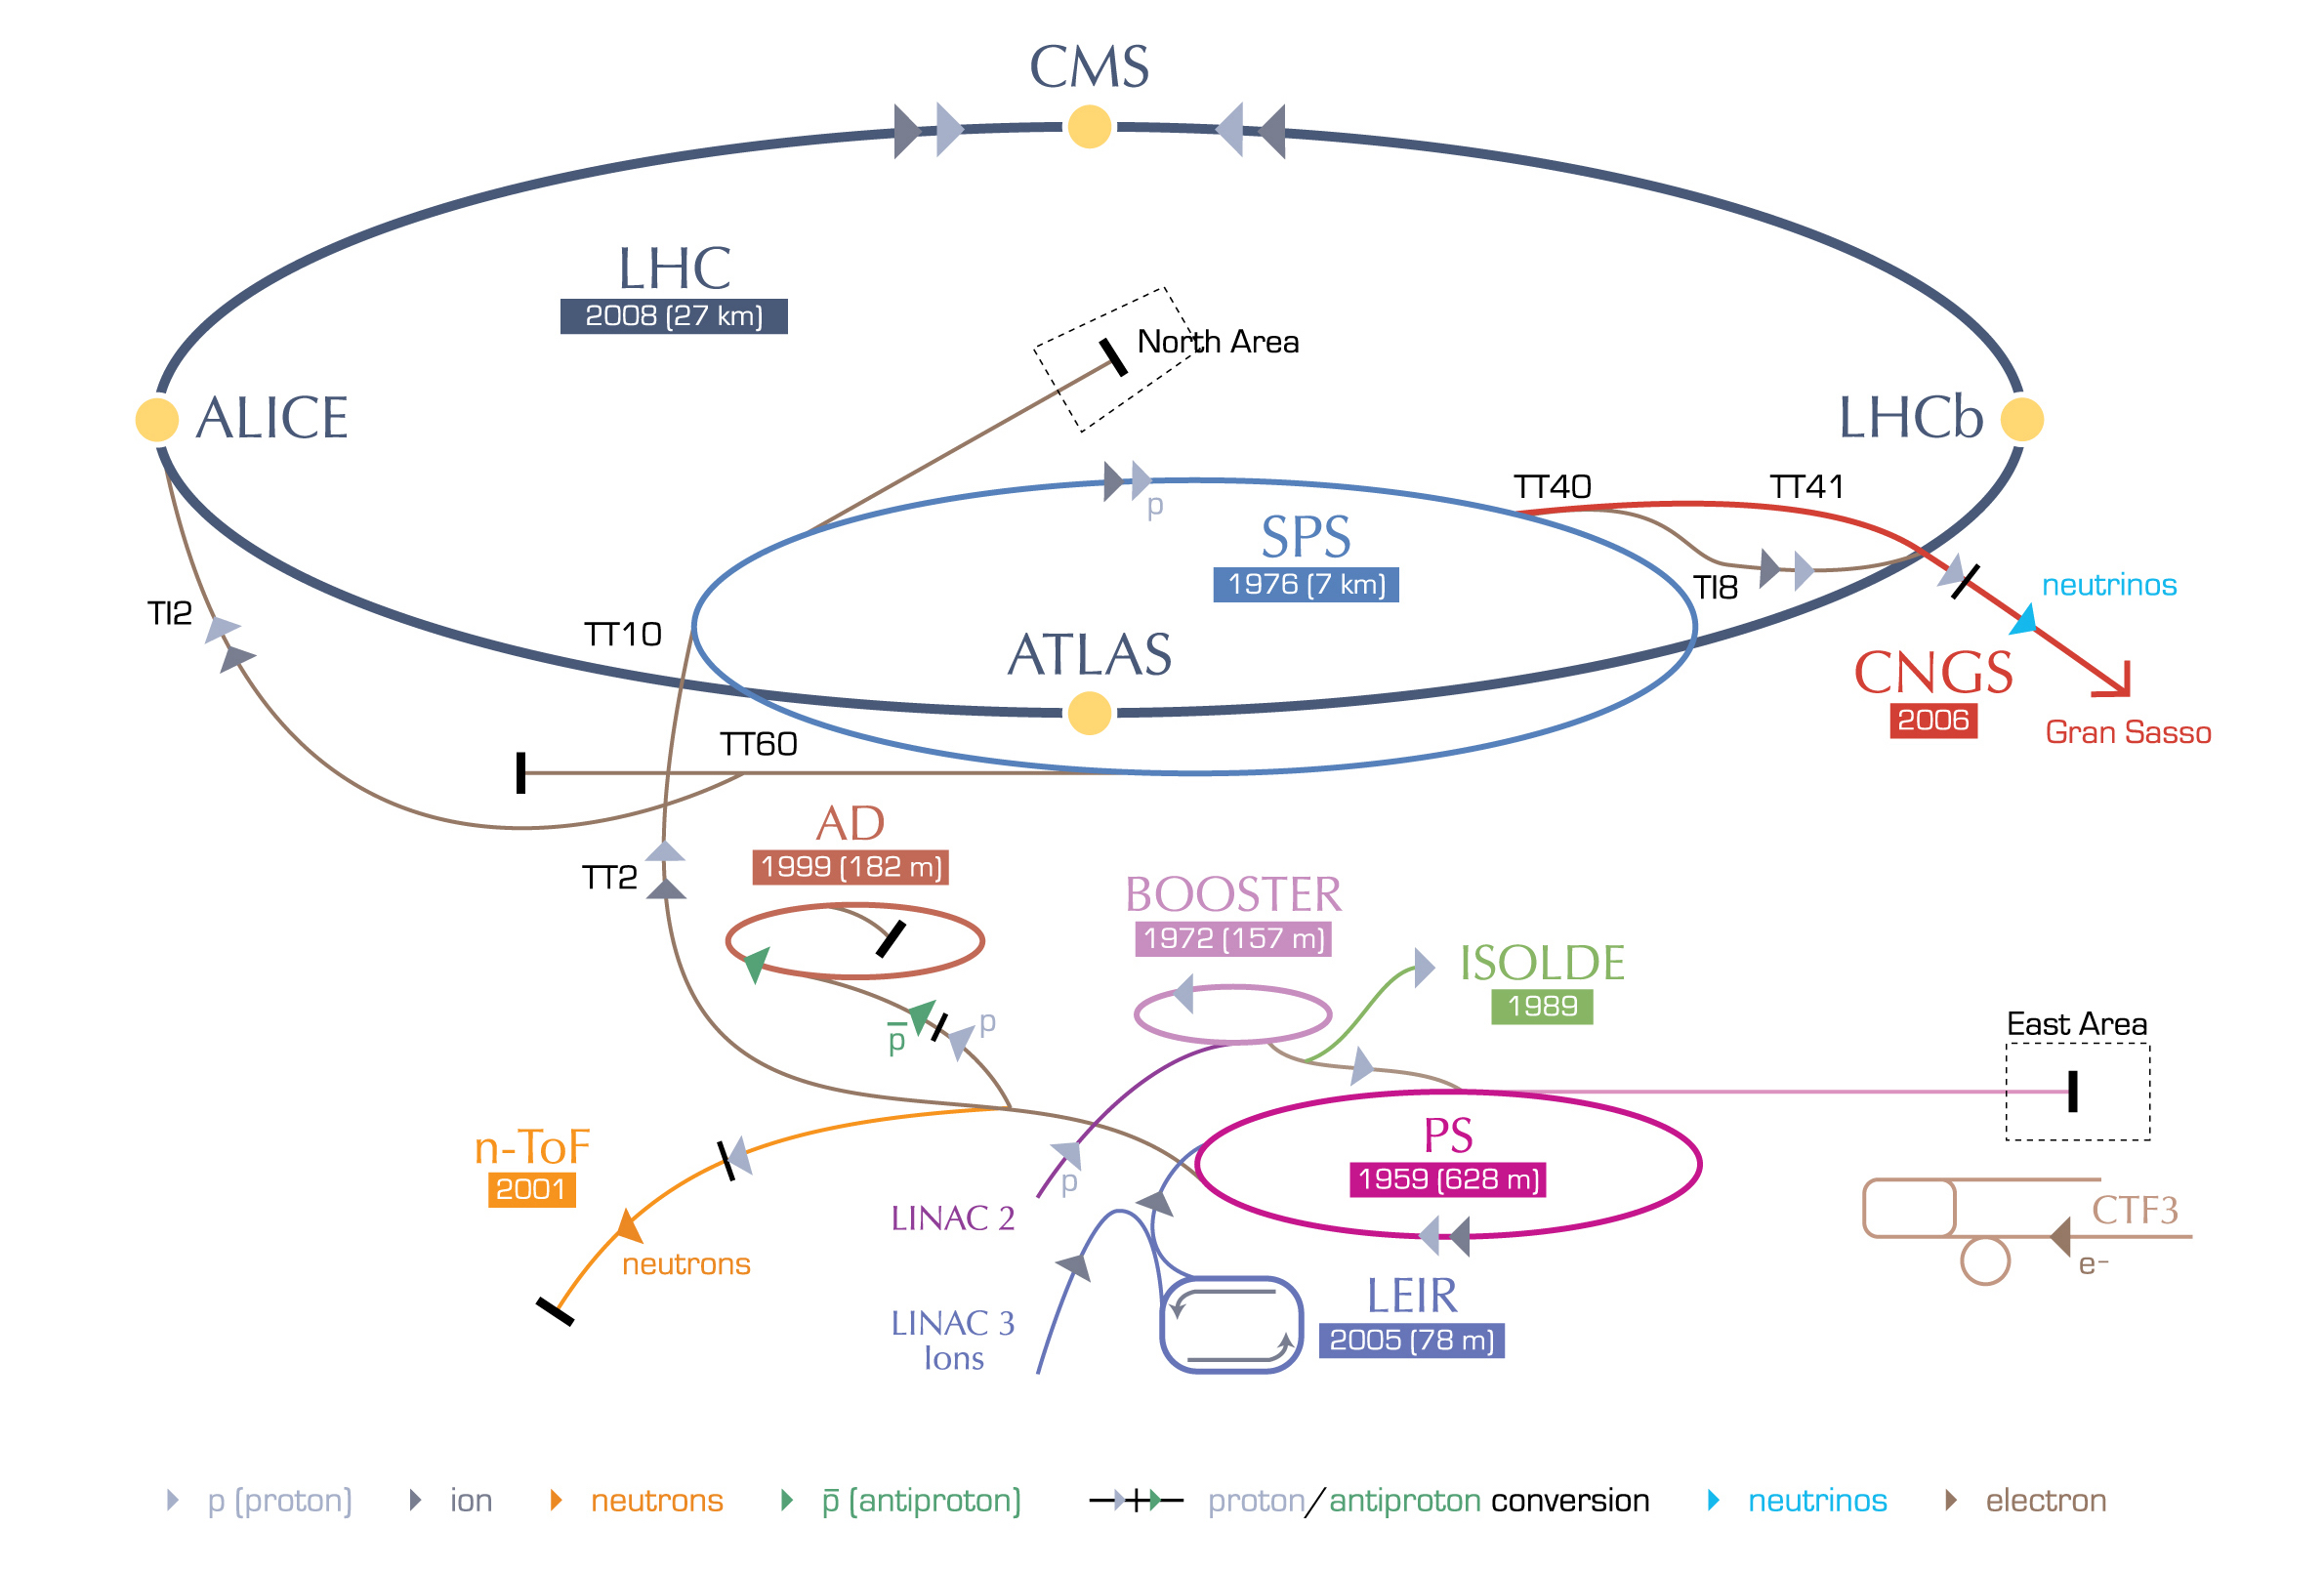
\includegraphics{figures/experiment/accelerator-complex.jpg}
    \newImageResize{figures/experiment/accelerator-complex.jpg}
    \caption{Illustration of the accelerator complex at CERN, including the Linac2, BOOSTER, PS, and SPS that serve as pre-accelerators before the protons are injected into the LHC. Adapted from \ccite{Christiane:1260465}.}
    \label{fig:accelerator-complex}
\end{figure}







\section{The ATLAS Experiment}
The ATLAS experiment is operated by a community of about 3000 scientific authors from 181 institutions and 41 countries~\cite{AtlasCollab}, making it one of the largest scientific collaborations in the world.
This section first provides an overview of the detection principles used to measure the various products of the $pp$ collision events and gives detailed information on the detector setup thereafter.

\subsection{Detection principles}
\label{subsec:measurement-principles}
Different types of particles, such as electrons, muons, or hadrons, originate from the $pp$ collisions and are measured in the ATLAS detector using two main methods: by detecting their trajectories, a method known as \emph{tracking}, and by measuring their energy via total absorption, a principle known as \emph{calorimetry}.

\subsubsection{Tracking}
%To reconstruct the trajectories of charged particles in the ATLAS detector, 
Tracks from charged particles can be reconstructed by measuring discrete space points and recognizing patterns.
The mostly non-destructive space point measurements are provided by detecting the signals (or \emph{hits}) left by traversing charged particles in finely segmented detector layers with known position. Different techniques are used in the ATLAS detector for this purpose:
\paragraph{Silicon semiconductor sensors} detect electron-hole pairs that are created in a p-n junction when a charged particle traverses the material. They can be segmented very finely and thus deliver precise spatial measurements.
\paragraph{Gas filled detectors} measure the current induced after a charged particle ionizes a gas via a wire connected at high voltage. The detectors consist of tubes or chambers with different arrangements of electrodes. Their main advantage is a low material cost which makes them useful for covering large areas. \\
% \paragraph{Transition radiation detectors} are based on gaseous ionization detectors and additionally measure the transition radiation from charged particles that traverse through material with different dielectric constants. The amount of transition radiation is sensitive to the Lorentz factor, which in combination with a momentum measurement provides the ability to measure the mass of a charged particle. This is useful input for particle identification. \\
\newline
To enable momentum measurements of charged particles, the tracking devices are immersed in magnetic fields that force the particles on a curved path. Their momenta can be determined from the radius of curvature of their reconstructed tracks. The resolution of the momentum measurement deteriorates linearly as the particle momentum increases.
%The following types of tracking devices are used in the ATLAS detector:
%The tracking devices are immersed in magnetic fields that force the charged particles on a curved path, allowing their momenta to be measured through the radius of their reconstructed tracks. 
% to bend the charged particles' trajectories. 
% This allows to measure the momentum of charged particles through the radius of their reconstructed track.

\subsubsection{Calorimetry}
%\emph{Calorimetry} can be defined as the detection principle to measure the energy of physics objects by fully absorbing them in blocks of instrumented material, called calorimeters.

Calorimeters measure the energy of particles by fully absorbing them and transferring their energy to electrical signals.
The ATLAS calorimeter is a so-called \emph{sampling calorimeter} where each of these tasks is handled by a dedicated material.
Layers of high-density \emph{passive material} are predominantly responsible for stopping the particles and are alternated with layers of \emph{active material} that focus on measuring the signals induced by the particles.
The total signal measured is proportional to the energy of the incident particle.

% comment from Mike (should be incorporated now!)
% This description is not strictly correct. It implies that the passive material stops the particles, which is true only as a whole. To be precise, there is also energy loss in the active material but of course much less.
% It is better to say that the absorber initiates showers, which are detected in the active layers. I see that you do this below.
% We can talk about how to re-word this if you want but I would rather you do it.


% Layers of \emph{passive material} stop the particles by initiating a process of repeated interactions with the detector material. They are alternated with layers of \emph{active material} that measure the signals deposited by the particles participating in the shower. 
% The ATLAS detector uses so-called \emph{sampling calorimeters} that comprise alternating layers of \emph{active material}, to actively measure the signals of the showering particles, and highly-dense \emph{passive material}, to initiate the showering and stop the particles.
\paragraph{Calorimeter showers}\mbox{}\\
As an incident particle interacts with the passive layers, a cascade of secondary particles forms.
Each secondary particle carries a fraction of the original energy and itself interacts with the calorimeter. This results in the formation of a \emph{calorimeter shower} that consists of particles with gradually decreasing energy as the shower evolves.
A distinction is made between \emph{electromagnetic showers} and \emph{hadronic showers}.

% The incident particles interact with the absorbers through several mechanisms which results in cascades of secondary particles known as \emph{showers}. 
Electromagnetic showers are initiated by electrons, positrons, and photons and are dominated by interactions through \emph{bremsstrahlung} (photon emission) and electron-positron \emph{pair-production}.
%The repeated process of emitting photons (bremsstrahlung) and producing electron-positron pairs (pair-production) forms a cascade of particles with gradually decreasing energy in the detector.
A material can be characterized by its radiation length, $X_0$, which denotes the length over which an electron or positron loses on average all but  $1/e$ of its energy via bremssstrahlung. Since the probability for interacting via bremsstrahlung is proportional to $1 / m^2$, where $m$ is the mass of the particle, muons deposit only a small fraction of their energy in the calorimeters and thus cannot be stopped.\footnote{While muons deposit only a small fraction of their energy in the calorimeters, it is important to consider these energy losses. This becomes more important as the energy of the muon increases, because the amount of energy that is lost due to bremsstrahlung increases with the energy of the muon. See also \cref{sec:muon-reconstruction}.}

Hadronic showers are more complex due to the rich nature of hadronic interactions. An incident hadron initiates showers by inelastic hadronic interactions with nuclei. In the process, several new particles are created, most of which are mesons.
The penetration depth of hadrons in a given material is characterized by their \emph{interaction length}, $\lambda$, which describes the length that a hadron travels on average without interacting.
More details on the characteristics of hadronic showers and their implications for calorimeter energy measurements are left to \cref{chap:calibration}.

\paragraph{Signal detection}\mbox{}\\
% The calorimeter showering as well as the active signal detection is described below.
% Incoming particles interact with the passive material, which initiates a process known as \emph{calorimeter showering}. The active material layers detect the signals of particles inside the showers. When the incoming particle is fully absorbed, the total collected signal is proportional to the initial energy of the particle. 
% \paragraph{Calorimeter showering} occurs when incident particles interact with the passive material through different mechanisms which results in cascades of secondary particles.
The active layers in the ATLAS calorimeter measure the signals from the particles participating in the showers. They consist of either \emph{liquid argon} (LAr) or plastic scintillating tiles.

The LAr-based systems are embedded in cryostats and measure the current induced by ionising particles. Readout electrodes are placed in the liquid and collect the charge within a timeframe of about \SI{450}{\nano\second}. The resulting signal is shown in \cref{fig:LAr-signal-pulse}. The pulse in the detector is first shaped to have a long negative tail in order to reduce the sensitivity to signals caused by $pp$ collisions from neighbouring bunches. The signal is then readout by sampling it four times at \SI{40}{\mega\hertz}. The pulse height is proportional to the energy of the traversing particle and energy calibrations are derived using data from dedicated runs~\cite{Abreu:1303004}.
% so that it can be converted to an energy measurement using calibrations derived from dedicated runs.~\cite{Abreu:1303004}

%In the LAr-based systems, that are embedded in cryostats, the incident charged particles ionize the liquid inducing a current that is measured at electrodes.
In the plastic scintillators, the energy of ionising particles is absorbed by the excitation of atoms and re-emitted in the form of light by the de-excitation of atoms. Also, photons produce light by exciting atoms after undergoing electron-positron pair production, Compton scattering, or photoelectric effect, depending on the energy of the photon.\footnote{Pair production dominates at higher energies larger than several \MeV, Compton scattering in the \MeV-range, and the photoelectric effect at lower energies below 1\,\MeV. The exact energy regime depends on the material.}.
The light is routed with wavelength shifting fibers to two photomultiplier tubes where it is converted to an electric pulse via the photoelectric effect. The pulse can be interpreted as an energy measurement with calibrations derived using data from dedicated runs~\cite{PERF-2007-01}.

\FloatBarrier
\begin{figure}[t]
    \newImageResizeHalf{figures/experiment/LAr-pulse-shape-red-dots.png}
    \caption{Signal pulse measured in the LAr detectors with and without pulse shaping. The large (red) dots indicate the positions at which the signal is ideally read out. Adapted from \ccite{Abreu:1303004}.}
    \label{fig:LAr-signal-pulse}
\end{figure}


\subsection{Overview of the ATLAS detector}
% An illustration of the detector is shown in \cref{fig:ATLASlayout}.
The ATLAS detector, illustrated in \cref{fig:ATLASlayout}, is \SI{44}{\meter} long, \SI{25}{\meter} high, and has a forward-backward symmetric geometry covering almost $4\pi$ in solid angle.
Several layers are arranged in a cylindrical structure around the beam axis.
%The different layers serve different functions and complement each other to form a detector system that is able to measure a wide range of physics processes.
The \emph{inner detector} (ID) is the innermost layer and serves as a tracking device surrounded by a large \emph{solenoid magnet}.
A large \emph{calorimeter system} is placed outside the solenoid and stops almost all electromagnetic and hadronically interacting particles.
The outermost part forms the \emph{muon spectrometer} (MS) which is designed to reconstruct muon tracks using large \emph{muon chambers} with \emph{toroid magnets} placed in between.
% to enable muon momentum measurements.

After introducing the ATLAS coordinate system below, the design and functionality of the different components is described in the remainder of this section.
While most of these sections are kept very brief, more details are provided on the calorimeter system, as it is the crucial component for the calibration measurement presented in the subsequent \cref{chap:calibration}.
More information about the ATLAS detector can be found in \ccite{PERF-2007-01}, which this section heavily relies on.

%Some of the detector components are also used to trigger on interesting physics events which is discussed thereafter.
%After describing the ATLAS coordinate system, a description of the tracking devices, the ID and the MS, followed by details on the calorimeter system.
%A combination of these subsystems is used to trigger on interesting physics events which is discussed thereafter.
%This section concludes with a description of the ATLAS simulation infrastructure. 

\begin{sidewaysfigure}
    \newImageResizeCustom{0.8}{figures/experiment/ATLASdetector.jpg}
    \caption[Schematic of the ATLAS detector showing the various subsystems.]{Schematic of the ATLAS detector showing the various subsystems.
        The innermost layers are used for tracking and consist of the silicon \emph{pixel detector}, the silicon \emph{semiconductor tracker}, and the \emph{transition radiation tracker}.
        They are surrounded by a large \emph{solenoid magnet}.
        The calorimeter system is placed outside the solenoid and includes the \emph{LAr electromagnetic calorimeters}, the hadronic \emph{tile calorimeters}, the \emph{LAr hadronic end-caps}, and the \emph{LAr forward calorimeters}.
        The outermost part forms the muon spectrometer which is designed to reconstruct muon tracks, using large \emph{muon chambers}, and is placed in between \emph{toroid magnets}. Taken from \ccite{PERF-2007-01}.}
    \label{fig:ATLASlayout}
\end{sidewaysfigure}

\subsection{The ATLAS coordinate system}
The ATLAS experiment uses a right-handed cartesian coordinate system to describe the hard-scattering processes. The origin is set at the nominal interaction point, which is at the geometrical centre of the ATLAS detector. The $z$-axis is along the beam direction, the $y$-axis points upwards, and the $x$-axis points to the centre of the LHC. The azimuthal angle $\phi$ is measured against the $x$-axis in the $x$-$y$ plane and the polar angle $\theta$ is the angle taken from the beam axis.
Final-state particles of $pp$ collision events are often Lorentz-boosted along the $z$-axis.
This is why the transverse component of the energy, $\ETvec = \ET \hat{n}$, or momentum, $\pTvec = \pT \hat{n}$, are often considered. They are determined by the projection of the total energy or momentum onto the $x$-$y$ plane.
The position of a particle in the $z$-$y$ plane is typically described with the \emph{pseudorapidity} $\eta$, defined as\footnote{For massive objects the \emph{rapidity} $y = \frac{1}{2} \text{ln} \left( \frac{E + p_Z }{E-p_z} \right)$ is used, where $E$ is the energy and $p_z$ the momentum in $z$-direction. The rapidity is approximated by the pseudorapidity for $m \ll E$, which is typically the case in for physics objects in high energy physics.}
\begin{equation}
    \eta = - \text{ln} \left( \tan \left( \frac{\theta}{2} \right) \right).
\end{equation}
This allows for an angular distance measurement $\Delta R$ between particles,
\begin{equation}
    \label{eq:delta-r}
    \Delta R = \sqrt{ \left( \Delta \eta \right) ^2 + \left( \Delta \phi \right) ^2 },
\end{equation}
that is invariant under Lorentz transformations along the $z$-axis.

% Comment Bernd
% Did you want to mention here are boosts along z are very common in pp colisons (which motivates this choice of coordinates)

\subsection{The inner detector}
\label{subsec:inner-detector}
%Charged-particle tracks stemming from the hard scatter can be reconstructed by recognizing patterns in the hits detected in the ID. 
The ID provides information about the charged-particle positions as close as \SI{27.5}{\milli\meter} to the interaction point.
Tracks reconstructed from ID hits are used for momentum measurements, impact parameter determination, as well as primary and secondary vertexing.
%Hits are detected by layers of different silicon-based semiconductor detectors as well as gaseous ionization tubes, see \cref{subsec:measurement-principles}. 
A schematic view of the ID is shown in \cref{fig:ATLASinnerdetector}.
In the central (barrel) region the tracking detectors are arranged in cylinders around the beam axis, while in the end-cap regions, the different layers are placed on disks perpendicular to the beam axis.
The ID covers a range \absetaST{2.5} and is immersed in a \SI{2}{\tesla} magnetic field that is provided by a \SI{5.8}{\m} long solenoid magnet.
The first tracking layer in the barrel is the insertable $b$-layer (IBL)~\cite{ATLAS-TDR-19,PIX-2018-001}, that was installed before \RunTwo and is especially important for the reconstruction of the interaction vertices.
Three layers of silicon \emph{pixels} in the barrel and each end-cap typically provide four space points for each charged particle.
Four layers (nine layers) of silicon-microstrip \emph{semiconductor trackers} (SCT) in the barrel (each end-cap) are composed of double layers of strips arranged at an angle of \SI{40}{\milli\radian} relative to each other. Four double layers are crossed by each track to provide additional four space points.
The fine granularity of the pixel and microstrip sensors provide high-precision measurements with resolutions in $R$-$\phi \times z$ ($R$-$\phi \times R$) of $10 \times 115\,\mu\text{m}$ and $17 \times 580\,\mu\text{m}$ for the pixel and microstrip barrels (end-caps), respectively.
The \emph{transition radiation tracker} TRT consists of a large number of straw tubes filled with xenon-based gas that provide on average 36 additional hits. The TRT covers a range \absetaST{2.0} and provides information in only the $R$-$\phi$ plane with a resolution of \SI{130}{\micro\meter}.
Apart from the position measurement, the TRT also generates and detects the amount of transition radiation, that is produced by high-energy charged particles when crossing two media of different dielectric constants. For this purpose, the TRT is interleaved with fibres and foils that provide the transition-radiation photons, which helps to differentiate electrons from charged pions.

% FROM MIKE:
% It would be good to add a couple of sentences to explain what TR is and how it is generated, e.g. there is a radiator in the detector.
% But don’t go overboard and describe the guts of TR generation. It is sufficient to say that it is a relativistic effect that is important only for electrons in ATLAS.

\FloatBarrier
\begin{sidewaysfigure}[t]
    %\resizebox{\textwidth}{!}{
    \subfloat[central region]{
        %\newImageScale{figures/experiment/ATLASinnerdetector.pdf}{.105}
        \newImageScale{figures/experiment/ATLASinnerdetector.pdf}{.155}
    }
    \subfloat[end-cap region]{
        \newImageScale{figures/experiment/ATLASinnerdetectorendcap.png}{.135}
        %\newImageScale{figures/experiment/ATLASinnerdetectorendcap.png}{.095}
    }
    %   }
    \caption{Schematic of the ATLAS inner detector in (a) the central region and (b) the end-cap region, showing the different systems: the IBL (not shown for the end-cap region), the pixel detector, the SCT, and the TRT. Taken from Refs.~\cite{ATL-PHYS-PUB-2015-009} and~\cite{PERF-2007-01}, respectively.}
    \label{fig:ATLASinnerdetector}
\end{sidewaysfigure}




% • They are versatile detectors. Although originally conceived as devices for energy measurement, they can be used to determine the shower position and direction, to identify
% different particles (for instance to distinguish electrons and photons from pions and
% muons on the basis of their different interactions with the detector), and to measure the
% arrival time of the particle. Calorimeters are also commonly used for trigger purposes,
% since they can provide fast signals that are easy to process and to interpret

\subsection{The calorimeter system}
\label{subsec:calorimeter}
The primary task of the ATLAS sampling calorimeter is to measure the energy of particles, but it is also sensitive to the position and direction of incident particles. The latter is enabled by the segmentation of the calorimeter into different cells in the $\eta-\phi$ plane and into several layers in the longitudinal direction.
This also allows quantifying other characteristics of the showers, which is used for particle identification (see \cref{chap:objects}).
The calorimeter signals provide fast information, which makes them also suitable for trigger purposes, which is described further below.

A schematic view of the calorimeter system is shown in \cref{fig:ATLAScalorimeters}.
It can be divided into a \emph{LAr electromagnetic calorimeter} (ECAL), that targets the measurement of electromagnetic showers, and a hadronic calorimeter, that measures and contains hadronic activity. The hadronic calorimeter is further subdivided into the scintillator \emph{tile calorimeter}, the \emph{LAr hadronic end-caps} (HEC), and the \emph{LAr forward calorimeters} (Fcal).
The entire system covers a large angle of \absetaST{4.9} with different materials used in different \abseta regions due to changing conditions.
Depending on the \abseta region, the ECAL and hadronic calorimeter provide a stopping power of $22-38\,X_0$ and $7-10\,\lambda$, respectively.
This limits the level of punch-through to the muon system almost entirely, except for the irreducible level of muons and neutrinos. % remain irreducible. the irreducible level of muons and neutrinos.
A summary of the most important material characteristics of the different segments is shown in \cref{tab:calorimeter-characteristics}.
Details on the detector coverage and granularity are given in \cref{tab:ATLAScalorimeter-parameters}.

\FloatBarrier
\begin{table}[h!]
    \centering
    \begin{tabular}{l | l l l}
        \toprule
                                                 & Active material               & Passive material         & Coverage                \\
        \midrule
        %LAr electromagnetic calorimeter barrel &  liquid argon     & lead             & $\approx 24 X_0$    & \absetaST{1.475}         \\
        %LAr electromagnetic calorimeter end-cap &  liquid argon     & lead             & $\approx 22 X_0$    & \absetaBT{1.375}{3.2}    \\
        LAr electromagnetic                      & \multirow{2}{*}{Liquid argon} & \multirow{2}{*}{Lead}    & \multirow{2}{*}{\absetaST{3.2}} \\
        calorimeter                              &                               &                          &                                 \\
        \midrule
        Tile calorimeter                         & Plastic scintillators                 & Steel                    & \absetaST{1.7}                  \\
        \midrule
        LAr hadronic end-caps                    & Liquid argon                  & Copper                   & \absetaBT{1.5}{3.2}             \\
        \midrule
        \multirow{2}{*}{LAr forward calorimeter} & \multirow{2}{*}{Liquid argon} & Copper (1st layer)       & \multirow{2}{*}{\absetaBT{3.1}{4.9}}             \\
                                                 &                               & Tungsten (2nd/3rd layer) &             \\
        \bottomrule
    \end{tabular}
    \caption[Characteristics of the different calorimeter systems of the ATLAS detector.]{
        Characteristics of the different calorimeter systems of the ATLAS detector, including the active and passive material used, and their \abseta coverage. Taken from \ccite{PERF-2007-01}.}
    \label{tab:calorimeter-characteristics}
\end{table}
%%%%%%%%%%%%%%%%%%%%%%%%%%%%%%%%%%%%%%%%%%%%%%%%%%%%%%%%%%%%%%%%
% Version with stopping power


% \begin{table}
%     \centering
%     \begin{tabular}{l | l l l l}
%         \toprule
%                                                  & Active material               & Passive material      & Stopping power                          & \abseta coverage                     \\
%         \midrule
%         %LAr electromagnetic calorimeter barrel &  liquid argon     & lead             & $\approx 24 X_0$    & \absetaST{1.475}         \\
%         %LAr electromagnetic calorimeter end-cap &  liquid argon     & lead             & $\approx 22 X_0$    & \absetaBT{1.375}{3.2}    \\
%         LAr electromagnetic                      & \multirow{2}{*}{Liquid argon} & \multirow{2}{*}{lead} & \multirow{2}{*}{$\approx 22-38\,X_0$}   & \multirow{2}{*}{\absetaST{3.2}}      \\
%         calorimeter                              &                               &                       &                                         &                                      \\
%         \midrule
%         Tile calorimeter                         & Scintillators                 & Steel                 & $\approx 7-10\,\lambda$               & \absetaST{1.7}                       \\
%         \midrule
%         LAr hadronic end-caps                    & Liquid argon                  & Copper                & $\approx TBD\,\lambda$                 & \absetaBT{1.5}{3.2}                  \\
%         \midrule
%         \multirow{4}{*}{LAr forward calorimeter} & \multirow{4}{*}{Liquid argon} & Copper                & $\approx 28\,X_0$ /                     & \multirow{2}{*}{\absetaBT{3.1}{4.9}} \\
%                                                  &                               & (1st layer)           & $\approx 3\,\lambda$                  &                                      \\
%                                                  &                               & Tungsten              & \multirow{2}{*}{$\approx 7\,\lambda$} & \multirow{2}{*}{\absetaBT{3.1}{4.9}} \\
%                                                  &                               & (2nd/3rd layer)       &                                         &                                      \\
%         \bottomrule
%     \end{tabular}
%     \caption{
%         Characteristics of the different calorimeter systems, including the active and passive material that is used, the approximate stopping power in terms of either the radiation length ($X_0$) or interaction length ($\lambda_0$) depending on whether the system targets electromagnetic or hadronic showers, and the \abseta coverage.
%         The stopping power is given as a range as it strongly depends on the $\eta$ region. \cite{PERF-2007-01}}
%     \label{tab:calorimeter-characteristics}
% \end{table}

\subsubsection{LAr electromagnetic calorimeters}
The ECAL is arranged in an accordion-shaped structure to ensure full coverage in $\phi$.
It is subdivided into a barrel part covering \absetaST{1.475} and an end-cap on each side in the range \absetaBT{1.375}{3.2}.

The barrel consists of two identical segments along the $z$-axis with a small gap of \SI{4}{\milli\meter} in between at $z=0$. A schematic of one of the barrel modules is shown in \cref{fig:ATLASmodules-a}. Each module is segmented in three layers in depth with varying granularity.
The first layer is finely segmented in $\Delta \eta$ which provides essential inputs for photon and neutral pion identification. The second layer is finer in $\Delta \phi$ and larger in depth and measures the bulk of the electromagnetic showers. The third and coarsest layer in $\Delta \eta$ is designed to measure the broad tail of the electromagnetic showers.
%Together, the three segments provide a stopping power of 24 radiation lengths ($X_0$) 
The high granularity provides valuable space point measurements in addition to the data from the ID, reduces the sensitivity to \pileup, and allows handling of large collision rates.

% Comment MIKE: It is also a matter of rate capability and reducing sensitivity to pileup.

% Previously more precise but too many numbers
% The first layer provides high resolution in $\Delta \eta$ with cell sizes of only $0.025 / 8 \times 0.1$ in $\Delta \eta \times \Delta \phi$. This provides essential inputs for photon and pion identification. The second layer measures the bulk of the electromagnetic showers and is finer in $\Delta \phi$ with cell sizes of $0.025 \times 0.025$ in $\Delta \eta \times \Delta \phi$. The third and coarsest layer in $\Delta \eta$ is designed to measuring the broad tail of the electromagnetic showers.
%Together, the three segments provide a stopping power of 24 radiation lengths ($X_0$) 
%The high granularity provides valuable space point measurements in addition to the data from the ID.

% - Accordion-shaped sampling detector (to provide full coverage in eta) with lead as absorber and LAr as active material.
% - EM cal with barrel in eta < 1.475 and end-cap 1.375 < eta < 3.2. 
% - Barrel has small gap of (4 mm) at z = 0. 
% - barrel module Shown in Figure. Three layers with varying granularity very useful for additional position measurement.
In the transition region between the barrel and end-caps (\absetaBT{1.37}{1.52}), also known as the ``crack'', there is a lot of material amounting to several $X_0$ in front of the calorimeter, which renders photon and electron identification difficult.

The end-caps consist of wheels placed on each side of the barrel.
They are composed of three layers in depth for the range \absetaST{2.5} and two layers for \absetaBT{2.5}{3.2} with varying thickness of the lead absorber. Details on the readout granularity is shown in \cref{tab:ATLAScalorimeter-parameters}.

To account for the energy that particles lose upstream of the ECAL, when traversing the ID and solenoid magnet, a presampler consisting of a thin LAr layer is placed in front of the ECAL in the range \absetaST{1.8}.

% - end-caps are two wheels. 
% - Transition region between barrel and endcap known as "crack", rendering photon and electron identification difficult. 
% - "lead thickness optimized has three segments in eta < 2.5 and two section in depth for eta > 2.5."
% - Presampler: "to correct for energy lost by electrons and photons upstream of the calorimeter for eta < 1.8 presampler detector consisting of a thin LAr layer of 1.1cm (0.5cm) thickness in barrel (end-cap)."
% "correct energy losses due to material in inner detector."
% "account for energy lost by electrons and photons traversing the ID and solenoid"
% - high-resolution measurement of electrons, photons.

\subsubsection{Hadronic tile calorimeter}
The hadronic tile calorimeter consists of a \emph{tile barrel}, that is placed directly outside the ECAL and extends to \absetaST{1.0}, and a \emph{tile extended barrel} on each side, covering \absetaBT{0.7}{1.7}.
Their granularity is much coarser than that of the ECAL (see \cref{tab:ATLAScalorimeter-parameters}).
%They provide a stopping power of around 7-10 interaction lengths depending on the $\eta$ region.
%The tile barrel surrounds the barrel of the ECAL and uses steel as absorber with scintillator tiles in between. 

A single module of the tile barrel is shown in \cref{fig:ATLASmodules-b}, depicting the alternating layers of plastic scintillator and steel. The scintillating light induced by traversing particles in the scintillators is collected at photomultipliers mounted on the tile edges via wavelength-shifting fibers. This allows for almost perfect $\phi$ coverage.

\subsubsection{LAr hadronic end-caps}
The HEC provides a coverage of \absetaBT{1.5}{3.2} and is segmented in two layers in depth. It consists of one end-cap wheel on each side of the detector. See Table 3.3 for details of the design.

\subsubsection{LAr forward calorimeter}
At very large angles (\absetaBT{3.1}{4.9}) the calorimeter needs to be especially resistant against radiation. The FCal consists of three thick absorber layers. The first layer targets measurements of electromagnetic showers, the second two provide necessary stopping power for hadrons.

% - LAr forward cals for both EM and HAD up to eta = 4.9. 
% - need to be especially resistant against radiation
% - 10 interaction lengths with three high-density modules per end-cap.
% - first is copper for EM measurements, the other two made out of tungsten for hadrons.



\begin{figure}
    \newImageScale{figures/experiment/ATLAScalorimeters.jpg}{.3}
    \caption[Schematic of the ATLAS calorimeters showing the different subcomponents.]{Schematic of the ATLAS calorimeters showing the different subcomponents. Details on are provided in the text. Taken from \ccite{PERF-2007-01}.}
    \label{fig:ATLAScalorimeters}
\end{figure}

\begin{figure}
    \subfloat[]{
        \newImageResizeCustom{0.53}{figures/experiment/barrel_module.png}
        \label{fig:ATLASmodules-a}
    }
    \subfloat[]{
        \newImageResizeCustom{0.43}{figures/experiment/tile_module_readout.png}
        \label{fig:ATLASmodules-b}
    }
    \caption{(a) Schematic of a single module of the electromagnetic calorimeter illustrating the different layers and their changing granularity as well as an indication of the accordion-like shape. (b) Schematic of a single module of the hadronic tile calorimeter showing the optical readout channels. Taken from \ccite{PERF-2007-01}.}
    \label{fig:ATLASmodules}
\end{figure}

\begin{table}
    \newImageResize{figures/experiment/calorimeter-specs.png}
    \caption{Main parameters of the calorimeter system. Taken from \ccite{PERF-2007-01}.}
    \label{tab:ATLAScalorimeter-parameters}
\end{table}



\subsection{The Muon Spectrometer}
Muons are minimum-ionising particles and escape the calorimeter system.
%Therefore, a large MS forms the outermost part of the ATLAS detector. 
The main purpose of the large MS therefore is to measure muon-track hits for muon reconstruction but also to provide information of a potential muon candidate to the trigger system.
\Cref{fig:ATLASmuonspectrometer} shows the MS including the large superconducting toroid magnets that are located in between several gaseous muon chambers.
The 8 barrel toroid magnets and 16 end-cap magnets cover the range \absetaST{1.4} and \absetaBT{1.6}{2.7}, respectively. They provide magnetic bending power of \numrange{0.5}{1}\,T to measure the muons' momenta. Precision-tracking chambers operate with an argon-based mixture and are arranged in three layers in both the barrel and end-cap regions. They cover a range \absetaST{2.7} and mostly consist of \emph{Monitored drift tubes}, that provide six to eight $\eta$ measurements. Only the innermost layer at \absetaBT{2}{2.7} is made out of multiwire proportional chambers called \emph{Cathode strip chambers} that are more resistant to radiation damage. They provide four space points in the $\eta$-$\phi$ plane. The detector chambers with fast readouts consist of \emph{Resistive-plate chambers} (RPCs) in the central-region within \absetaST{1.05} and \emph{Thin-gap chambers} (TGCs) in the end-cap regions at \absetaBT{1.05}{2.4}.
Their main purpose is to provide information to the Level 1 trigger system (discussed below in \cref{sec:trigger-system}), but also to provide information complementary to the precision trackers to allow for a three-dimensional track reconstruction of the muon candidates.

% They provide information about traversing muons to the L1 trigger system that is discussed below within \numrange{15}{25}\,ns.
%The RPCs are gaseous parallel electrode-plates without a wire and 

\FloatBarrier
\begin{figure}[t]
    \newImageScale{figures/experiment/ATLASmuondetector.png}{.15}
    \caption{Schematic of the ATLAS muon spectrometer. Taken from \ccite{PERF-2007-01}.}
    \label{fig:ATLASmuonspectrometer}
\end{figure}



\subsection{Trigger System}
\label{sec:trigger-system}
It is technically not feasible to store the detector response for each collision event that occurs every \SI{25}{\nano\second}.
A dedicated trigger system therefore makes fast decisions and selects only events for readout which exhibit interesting features.
The selections are based on the available data from various detector subsystems.
% It uses different detector systems and reduces the rate of events selected for readout to \SI{1}{\kilo\hertz}. 
% and selects them for readout. 
%The nominal rate of collision events of produce much more data to be stored than is technically feasible. 
The \RunTwo trigger system consists of a two-stage approach:
The hardware-based \emph{Level-1} (L1) trigger reduces the rate of collision events from \SI{40}{\mega\hertz} to \SI{100}{\kilo\hertz} and provides inputs to the software-based \emph{High-level trigger} (HLT), implemented in a large dedicated computer farm, which makes further selections to reduce the rate to around \SI{1000}{\hertz}.

The L1 trigger uses information from both, the full MS and the entire calorimeter system but with reduced granularity.
The muon trigger chambers (RPCs and TGCs) detect muons with high transverse momenta, while the showering information from the calorimeters is used to search for electrons, photons, jets, hadronically decaying \tauleptons, as well large missing or total transverse energy.\footnote{The definition and reconstruction procedure of these physics objects are described in \cref{chap:objects}.}
By adjusting the identification criteria and thresholds used for the different objects, the trigger rates for different event signatures can be controlled.
Events with certain signatures such as high-\pT jets or large missing transverse energy often occur more frequently than desired for readout. In these cases the related triggers can be \emph{prescaled} by a certain factor to only select one out of many events of that type\footnote{The decision which event is read out is randomized to avoid possible biases}. This enables a controlled data collection as running conditions change.\footnote{All events with at least one identified electron, muon or large missing transverse momentum are \emph{unprescaled}.}
In addition to reducing the event rate, the L1 trigger defines \emph{Regions-of-interest} (ROIs) in the $\eta$-$\phi$ plane to locate the interesting features.
The HLT analyzes the detector signals in the ROIs performing ``offline-like'' full event reconstruction using all detector subsystems with their full granularity. The ROIs typically make up around \SI{2}{\percent} of the total event data.
The events selected by the HLT are subsequently stored to disk.
More information on the ATLAS trigger system can be found in \ccite{ATLAS-TDR-16,ATLAS-TDR-12,PERF-2007-01}.

% Goal:
% - Nominal rate of collisions much higher than the maximum that can be stored
% - Most types of events not interesting
% - Trigger / select the interesting events for read out
% Physics / Technology Exploited:
% - Different detector systems with fast readout at play
% Technical Details:
% - L1 trigger defines ROIs in eta - phi space where it detects interesting features
% - High-level trigger (HLT) analyzes ROIs and makes further selections
% - So-called pre-scaling available
% From ATLAS paper: "The L1 trigger searches for signatures from high-pT muons, electrons/photons, jets, and tau-leptons decaying into hadrons. It also selects events with large missing transverse energy (Emiss)
% and large total transverse energy. The L1 trigger uses reduced-granularity information from a
% subset of detectors: the Resistive Plate Chambers (RPC) and Thin-Gap Chambers (TGC) for high-
% pT muons, and all the calorimeter sub-systems for electromagnetic clusters, jets, tau-leptons, Emiss, T
% and large total transverse energy."
% From Arnold: "
% The L1 trigger decision is based on coarse-granularity measurements provided by a limited set of the detector subsystems, i.e. the EM and hadronic calorimeters as well as the muon trigger chambers, RPC and TGC."
% - HLT further processes inputs from L1 using all detector subsystem with their full granularity. Only the ROIs identified by the L1 trigger are processed.
% - In the HLT only the ROIs identified by the L1 are further analyzed, but using all detector subsystems with their full granularity.


\subsection{Detector simulation}
%Simulations of the ATLAS detector are required in order to generate full Monte Carlo events that can be compared to actual experimental data.
The ATLAS detector simulation is based on \textsc{Geant4}~\cite{Agostinelli:2002hh}.
The simulations considers all aspects of the ATLAS detector such as the response of each individual detector system, the effect of material placed throughout the detector, detector imperfections, as well as data and trigger conditions.
% From Deep Learning and its applications in physics
%In the language of statistics and machine learning, the full simulation chain would be considered a generative model for the data as they can be used to generate synthetic data of the same complexity and format as the actual collision data.
%Due to the complexity of the experiment a \emph{full simulation} is a very computing-intensive process. The ATLAS simulation infrastructure also allows for \emph{fast simulations} using simplified descriptions of the detector systems. This provides the opportunity for lower processing times with the drawback of decreased accuracies.
The simulations produce data of the same complexity and format as the actual experimental data, so the same software can be used for further processing of the events.
More information on the ATLAS simulation infrastructure can be found in \ccite{ATLAS-TDR-17,SOFT-2010-01}.
%- full simulation of particle interaction with matter throughout detector 


\todo{should I mention the detectors that measure the luminosity?}
\section{Data Acquisition during 2015-2018}
\label{sec:run-2-data-taking}
The operation of the LHC during \RunTwo between April 2015 and December 2018 was a great success and even exceeded the goals set in terms of luminosity production. At a centre-of-mass energy of $\sqrt{s} = 13\,\TeV$, the peak instantaneous luminosity was more than twice as high as its design value reaching up to $\instLumi = \SI{2.1e34}{\per\cm\per\s}$ in 2018.
\Cref{fig:run-2-data-taking-a} shows the integrated luminosity delivered by the LHC (156\ifb), recorded by the ATLAS detector (147\ifb), and certified as being of ``good'' data quality (139\ifb).
The recorded luminosity reflects the small inefficiency of the data acquisition infrastructure as well as the fact that the ATLAS detector is fully activated for readout only after a short ramp-up period in the tracking detectors that is started once the LHC produces stable beam collisions.
The recorded data are further filtered before being considered for physics analyses.
An event is considered ``Good for Physics'' if all reconstructed objects satisfy certain data-quality requirements and if it was recorded at times when all relevant detector components were fully operational.
The integrated luminosity that is analyzed by physics analyses makes up 89\% of the total delivered luminosity.
More information on the data quality monitoring framework can be found in \ccite{DAPR-2018-01}.

Due to changing running conditions, the distribution of the mean number of interactions per bunch crossing varies between the years.
The distributions are shown in \cref{fig:run-2-data-taking-b}.
Noticeable is the double-peak structure of the data recorded in 2017.
An alternative beam production scheme had to be used because of an issue in the beam vacuum for some periods in this year\footnote{In 2017, during the replacement of a dipole magnet seven liters of air entered the beam vacuum. The water vapor froze at the interconnection of cell 16L2 which lead to unstable beams that were dumped early~\cite{Jimenez:2646067,Salvant:2646056}. More information can be found in \ccite{Steerenberg:2696126}.}. This resulted in particularly high pile-up conditions of up to 60-70 interactions per bunch crossing and thus the mentioned double-peak structure.
% In 2017, the LHC performance was hampered by the so-called 16L2 issue: frozen air in an interconnection between magnets in the arc connecting Point 1 (ATLAS) with Point 2 (ALICE)In 2017, the LHC performance was hampered by the so-called 16L2 issue: frozen air in an interconnection between magnets in the arc connecting Point 1 (ATLAS) with Point 2 (ALICE)
More details on the LHC running conditions during \RunTwo can be found in \ccite{Steerenberg:2696126}.

\begin{figure}[t]
    \subfloat[]{
        \newImageScale{figures/reconstruction/run2-lumi.pdf}{.38}
        \label{fig:run-2-data-taking-a}
    }
    \hspace{-3.95em}
    \subfloat[]{
        \newImageScale{figures/reconstruction/run2-pileup.pdf}{.38}
        \label{fig:run-2-data-taking-b}
    }
    \caption{(a) Collected luminosity and (b) Mean number of interactions per crossing for $pp$ collisions during \RunTwo of the LHC. More information is provided in the text. Taken from \ccite{PublicLumiResults}.}
    \label{fig:run-2-data-taking}
\end{figure}

% Caption from ATLAS (https://twiki.cern.ch/twiki/bin/view/AtlasPublic/LuminosityPublicResultsRun2#Multiple_Year_Collision_Plots)
% Number of Interactions per Crossing
% Shown is the luminosity-weighted distribution of the mean number of interactions per crossing for the 2018 pp collision data at 13 TeV centre-of-mass energy. All data recorded by ATLAS during stable beams is shown, and the integrated luminosity and the mean mu value are given in the figure. The mean number of interactions per crossing corresponds to the mean of the poisson distribution of the number of interactions per crossing calculated for each bunch. It is calculated from the instantaneous per bunch luminosity as μ=Lbunch x σinel / fr where Lbunch is the per bunch instantaneous luminosity, σinel is the inelastic cross section which we take to be 80 mb for 13 TeV collisions, and fr is the LHC revolution frequency. The luminosity shown represents the preliminary 13 TeV luminosity calibration for 2018, released in February 2019, that is based on van-der-Meer beam-separation scans. Data collected by ATLAS for the entire 2018 run through the end of October are shown.

% Total Integrated Luminosity and Data Quality in 2015-2018
% Cumulative luminosity versus time delivered to ATLAS (green), recorded by ATLAS (yellow), and certified to be good quality data (blue) during stable beams for pp collisions at 13 TeV centre-of-mass energy in 2015-2018. The complete pp data sample in 2018 is shown. The delivered luminosity accounts for the luminosity delivered from the start of stable beams until the LHC requests ATLAS to put the detector in a safe standby mode to allow a beam dump or beam studies. The recorded luminosity reflects the DAQ inefficiency, as well as the inefficiency of the so‐ called "warm start": when the stable beam flag is raised, the tracking detectors undergo a ramp of the high-voltage and, for the pixel system, turning on the preamplifiers. The data quality assessment shown corresponds to the All Good efficiency shown in the 2015-2018 Full Dataset DQ tables here. The All Good Data Quality criteria require all reconstructed physics objects to be of good data quality.
